\documentclass[a4paper]{article}
\usepackage[warn]{mathtext}
\usepackage[utf8]{inputenc}
\usepackage[T2A]{fontenc}
\usepackage[english,russian]{babel}
\usepackage{indentfirst}
\usepackage{misccorr}
\usepackage{subcaption}
\captionsetup{compatibility=false}
\usepackage{geometry}
\geometry{verbose,a4paper,tmargin=2cm,bmargin=2cm,lmargin=1.5cm,rmargin=1.5cm}
\usepackage{graphicx}
\usepackage{wrapfig}
\usepackage{amsmath}
\usepackage{fancyhdr}
\usepackage{floatflt}
\usepackage{float}
\usepackage{amssymb}
\usepackage{color}
\usepackage{lscape}
\usepackage{hvfloat}
\usepackage{amsfonts}
\usepackage{euscript}
\usepackage{newunicodechar}

\begin{document}

\begin{titlepage}
	\centering
	\vspace{5cm}
	{\scshape\LARGE Московский физико-технический институт \par}

	\vspace{3cm}
	{\scshape\Large Лабораторная работа № 4.6.2 \par}
	\vspace{1cm}
	{\huge\bfseries  Туннелирование на сверхвысоких частотах\par}
	\vspace{1cm}
	\vfill
\begin{flushright}
	{\large Выполнила студентка группы Б01-903}\par
	\vspace{0.3cm}
	{\LARGE Прохорова Юлия}
\end{flushright}
	
	\vfill

% Bottom of the page
	Долгопрудный, 2021 г.
\end{titlepage}



\newpage

%\tableofcontents

\newpage

\newcommand{\RNumb}[1]{\uppercase\expandafter{\romannumeral #1\relax}}

\pagestyle{fancy} 
\fancyhead{} 
\fancyhead[R]{Юлия Прохорова, Б01-903} 
\fancyhead[L]{4.6.2}
\fancyfoot[C]{\noindent\rule{\textwidth}{0.4pt} \thepage}

\section{Цель работы:} исследование явления проникновения электромагнитного поля во вторую среду при полном внетреннем отражении(туннелирование) и использование этого явления для создания интереференционных схем в СВЧ-диапазоне.  
	
\section{Оборудование:} генератор СВЧ-колебаний, излучающая и приемная рупорные антенны, детектор, две фтороплазмовые призмы, металлические зеркала, микроамперметр, плоскопараллельная пластина из фторопласта.

\section{Теоретическая часть}

Проникновение электромагнитных волн в менее плотную среду при полном внутреннем отражении ­ явление
той же природы, что и проникновение частиц в область, где их полная энергия оказывается меньше потенциальной энергии. Это явление изучается в квантовой физике и носит название туннельного эффекта.

    \begin{figure}[H]
		\begin{center}
		\label{graf_a}
		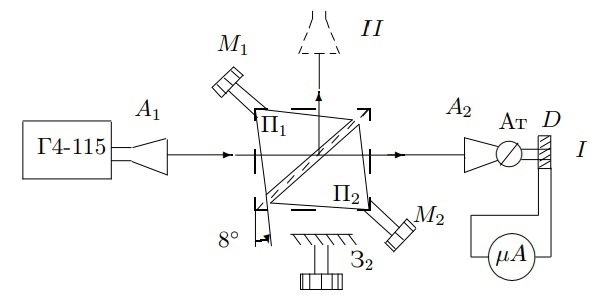
\includegraphics[scale=0.5]{2.jpg}
		\caption{Схема установки}
		\end{center}
	\end{figure}

Исследуем этот эффект ­ проникновение ЭМВ через воздушный зазор между диэлектрическими призмами
при полном внутреннем отражении на границе диэлектрик­воздух. Моделирование интерферометра Майкельсона с использованием этого эффекта и измерение длины волны излучения и показателя преломления фторопласта
для радиоволн миллиметрового диапазона.
Для измерения показателя преломления матриала призм мы установим пластину толщины $h$ из того же матриала, что и призмы ­ фторопласта. Имеем тогда приращение длины "оптического пути".

\begin{equation}
    \varDelta = 2h(n - 1)
\end{equation}

Данное приращение можно скомпенсировать, передвинув подвижное зеркало на необходимое расстояние
$\delta x$ :

\begin{equation}
    \delta = 2h(n - 1)
\end{equation}

Для толстых пластин, когда $\varDelta > \lambda$, необходимо учесть изменение порядка интерференции. Это можно сделать, зная приближенное значение преломления флоропласта ($n \approx 1,5$).

\section{Ход работы}

\subsection{Исследование туннелирование СВЧ волн.}

\begin{enumerate}
    \item Настроим генератор. Рабочая частота клистрона $35,93 - 35,99$ ГГц, мы настроили на - $35,96$ ГГц.
    \item Рассчитаем соответствующую длину волны для частоты - $\lambda = \frac{c}{\nu} = 8,34 \pm 0,01$ мм. 
    \item Можности соответствует - $38$ Вт (1 дел - 100 нА).
    \item Переставим приемник для регистрации отраженного света.  Получим зависимость для преломленного и отраженного света:
    
    \begin{figure}[H]
		\begin{center}
		\label{graf_a}
		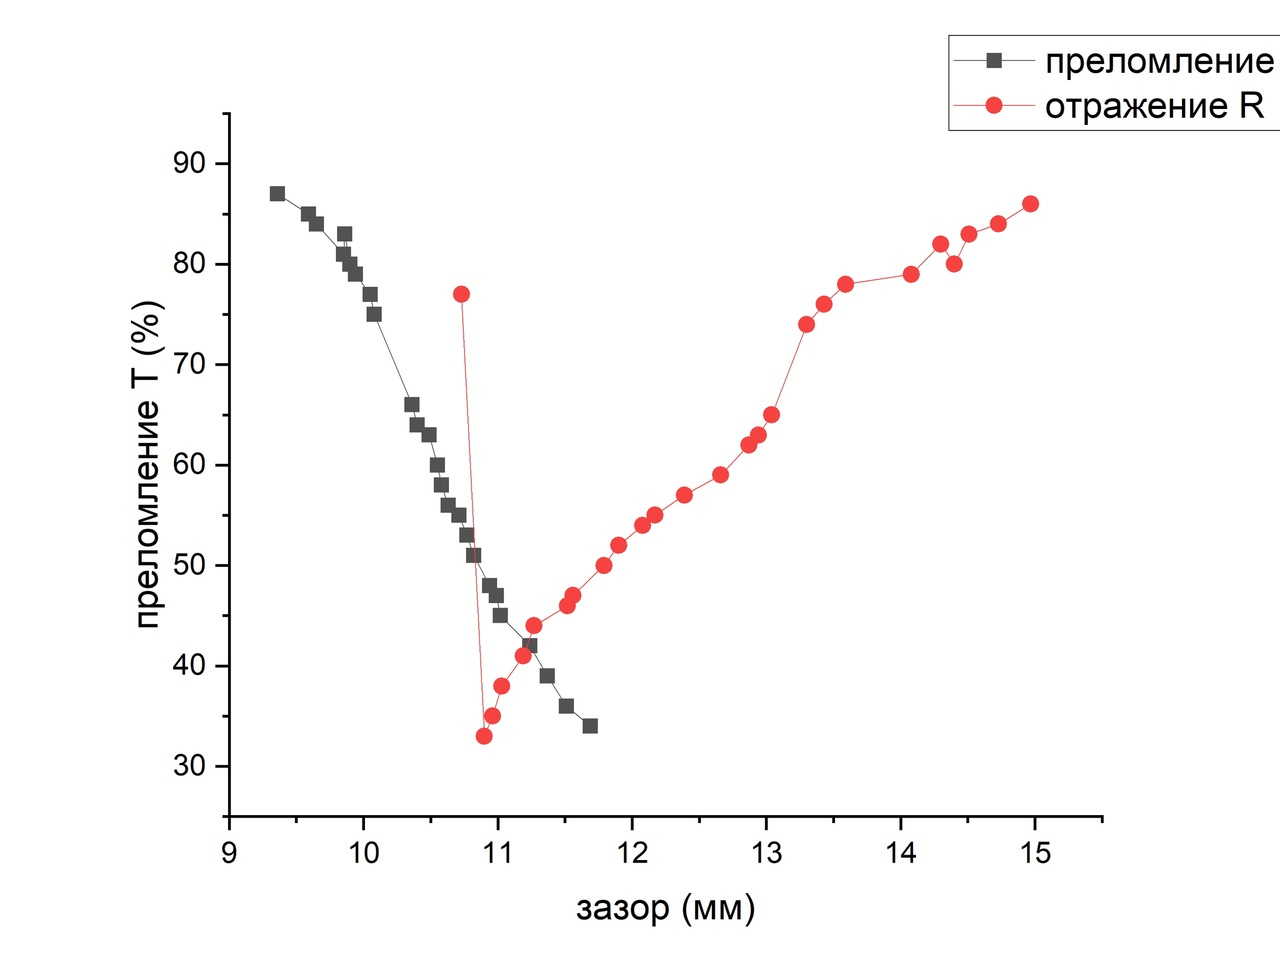
\includegraphics[scale=0.3]{3.jpg}
		\caption{Завиимость $T$ и $R$ от $l$}
		\end{center}
	\end{figure}

    \item Можно заметить, что по полученным данным $T + R \approx 1$.
    \item Далее построи график $ln(T) = f(z)$
    
    \begin{figure}[H]
		\begin{center}
		\label{graf_a}
		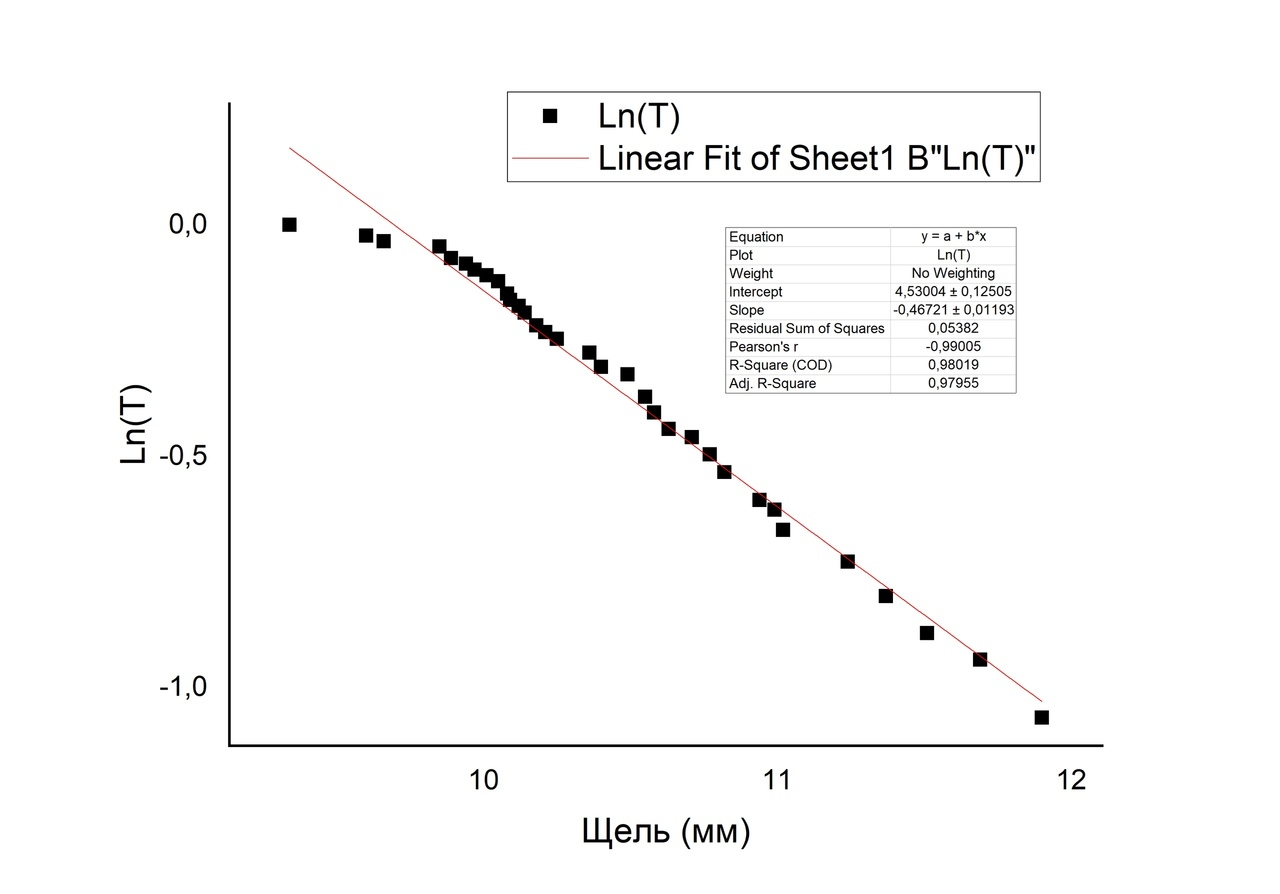
\includegraphics[scale=0.3]{1.jpg}
		\caption{$ln(T) = f(z)$}
		\end{center}
	\end{figure}

    \item Далее вычисляем показатель преломления $n$ с учетом того, что $\Lambda = 0,46 \pm 0.01$ и $\phi \approx \frac{\pi}{4}$:
    
    \begin{equation}
        n = \frac{1}{sin\phi}\sqrt{1+ \frac{1}{(4\pi\Lambda)^2}} = 1,4 \cdot 0,1 \; мм
    \end{equation}

    \item Полученное значение - хорошо согласуется с табличным значением - $1,46$
\end{enumerate}

\section{Интерферометр Майкельсона}

\begin{enumerate}
    \item Установим такой зазор, чтобы $T \approx R \approx 0,5 $. Соберем схему Майкельсона.
    \item Снимем зависимость силы тока от коодинаты подвижного зеркала. $ I = f(x)$. Получили зависимость:
    \item Вставим в пластину фторопласта $h = 6,2 $мм. Получили $\delta x 1,77$ мм.
    \item Рассчитаем показатель преломления:
    \begin{equation}
        n = 1 + \frac{\delta x}{h} = 1,3 \pm 0,1 мм
    \end{equation}

\end{enumerate}

\section{Вывод} 
 
В работе получена зависимость $T$ и $R$ от $l$ и $ln(T) = f(z)$. По первому графику подтвердилось соотношение $T + R \approx 1$, по второму получилось значение $n = 1.4 ± 0.1$ мм, совпадающее с табличным в пределах
погрешностей. Значение, измеренное интерферометром Майкельсона, оказалось далеким от правды. Возможно, мы сдвинули установку при измерении и из-за это получили неточные значения.

\end{document}